\chapter{Marco teórico}
\label{ch:marco}

\section{Descripción}

Toda tesis hace referencia a trabajos previos en el área y trabajos afines que
están directamente relacionados con lo planteado en el tesis.

Además, en el marco teórico debe aparecer la información absolutamente
necesaria para comprender la solución, y por eso es recomendable escribir
primero la solución (el siguiente capítulo), para ir anotando qué debe ser
explicado en el marco teórico.

\section{Generalidades}

Se recomienda revisar las guías de publicación de la \nt{IEEE} en
\url{http://www.ieee.org/publications_standards/publications/authors/authors_journals.html},
donde puede encontrar cómo hacer referencias bibliográficas correctamente, cómo
citar ecuaciones, tablas y figuras, etc.  

\subsection{Redacción}

La \nt{redacción} en todo el documento debe seguir un estilo científico
objetivo. Esto implica que se redacta de modo impersonal, sin utilizar primeras
personas del singular o del plural, y se evita el uso de cualquier tipo de
calificativo, sustituyéndolos siempre por datos concretos, vinculados a
referencias bibliográficas o datos experimentales. Los comparativos también
deben concretarse a hechos y datos, y nunca dejarse ``en el aire''. Por la
naturaleza de la tesis, el tiempo verbal es usualmente presente, no perdiendo
nunca de vista que se está explicando ``cómo hacer algo'', en vez de ``qué se
hizo''.

Las \nt{frases} deben ser cortas, y debe evitarse que el lector tenga que saltar
constantemente entre partes de la tesis, lo que implica una exposición lineal
clara, donde lo que se necesita ya ha sido explicado antes. Deben evitarse
redundancias y por tanto cada concepto se exponen en un único lugar.

Todo aspecto circunstancial es irrelevante para la tesis, es decir, si se ha
desarrollado en el laboratorio $X$, o en el curso $Y$, con el profesor $Z$, o
en la empresa $W$, el nombre de funciones o clases en su código, etc., es
información irrelevante para reproducir el experimento, y por lo tanto sobra.
Numeración del documento

La primera página de la tesis es la correspondiente a la introducción, así que
ésta debe ser la página 1. Desde la introducción, hasta antes de la
bibliografía, las unidades son ``Capítulos''. La bibliografía y anexos no se
consideran capítulos, así que ya no continúan con la misma numeración de los
capítulos (la paginación sí continua). Los índices, notación, glosario, etc. se
numeran con números romanos en minúscula (i,ii,iii,iv,v,vi...) y antes del
índice (portada, resúmenes, agradecimientos, hoja de evaluadores, etc.) las
páginas no llevan numeración. 

Esta plantilla LaTeX ya se ocupa de todo lo anterior.

\subsection{Ecuaciones}

Para citar \nt{ecuaciones} se utilizan paréntesis redondos, y no es necesario
emplear la palabra ``ecuación''. Por ejemplo ``Introduciendo en (4.2) los
resultados de (3.3) y (3.7) se obtiene ...''. La ecuación es parte del flujo de
texto y no un objeto flotante, así que no pueden emplearse como figuras. Cuando
se requiere la ecuación, allí se inserta.  

Es incorrecto redactar de la siguiente forma: \explain{MAL}

\textsl{La operación del transistor sin tomar en cuenta el efecto Early está
  dada por (\ref{eq:ej1}), donde el parámetro $\kappa$ está dado por
  (\ref{eq:ej2}).}

\begin{equation} \label{eq:ej1}
  I_{DS}
  =
  I_{n0} \frac{W}{L}e^{\kappa \frac{V_{GB}}{v_t}}
  \left[
    e^{-\frac{V_{SB}}{v_t}}
    -
    e^{-\frac{V_{DB}}{v_t}}
  \right]
\end{equation}

\begin{equation} \label{eq:ej2}
  \kappa = \frac{C_{ox}}{C_{ox}+C_{dep}}
\end{equation}

Lo anterior es incorrecto porque obliga al lector a estar buscando ecuaciones,
que pueden mostrarse directamente.  La única referenciación permitida es hacia
atrás.

La forma correcta de redactar lo anterior es: \chk{BIEN}

\textsl{La operación del transistor sin tomar en cuenta el efecto Early está
  dada por}
\begin{equation} \label{eq:ej3}
  I_{DS}
  =
  I_{n0} \frac{W}{L}e^{\kappa \frac{V_{GB}}{v_t}}
  \left[
    e^{-\frac{V_{SB}}{v_t}}
    -
    e^{-\frac{V_{DB}}{v_t}}
  \right]
\end{equation}
\textsl{donde el parámetro $\kappa$ es}
\begin{equation} \label{eq:ej4}
  \kappa = \frac{C_{ox}}{C_{ox}+C_{dep}}
\end{equation}

Así el flujo del texto guía al lector por las ecuaciones sin mayor esfuerzo.

Es recomendable numerar \emph{todas} las ecuaciones, de modo que en la revisión
del documento, o en futuras referencias a su documento de tesis todas las
ecuaciones puedan ser citadas sin requerir describir textualmente a cuál
ecuación se está haciendo referencia.

\subsection{Figuras}

Para el almacenamiento de imágenes existen dos tipos de formato: las imágenes
raster y las imágenes vectoriales.\index{imagen!raster}

\subsubsection{Imágenes raster}

Las imágenes raster son representadas por una rejilla de píxeles, en donde cada
píxel tiene un valor que representa al nivel de gris o el color. La
discretización espacial es ineludible, y la única forma de obtener buena
calidad es empleando tamaños grandes de la imagen que conduzcan a resoluciones
de al menos 300 puntos por pulgada en la impresión, lo que conlleva a archivos
de documentos de varios megabytes. Dentro de los formatos para almacenar
imágenes raster existen algunos con pérdida (como el JPEG) que producen en
imágenes sintéticas, como diagramas, estructuras ruidosas que dan una
apariencia de baja calidad a las figuras. Otros formatos (como PNG, BMP, TIFF o
GIF) no tiene pérdidas de información, pero los algoritmos de compresión no
pueden reducir el tamaño de las imágenes con los mismos factores de reducción
que los formatos con pérdidas. Este tipo de formatos debe utilizarse únicamente
para fotografías o capturas de escenas reales con cámaras digitales.

\subsubsection{Imágenes vectoriales}

\index{imagen!vectorial}
Las imágenes vectoriales \textbf{deben} ser empleadas en todo tipo de
diagrama. En ellas no se almacenan píxeles, sino las estructuras geométricas
que componen la figura como círculos (representado por posicion de su centro y
su radio), rectángulos (representados por sus esquinas), líneas, texto, etc. La
mayoría de programas para elaborar este tipo de diagramas, como Inkscape, XFig,
OpenOffice.org Draw, MS Visio, Adobe Illustrator, etc. proveen varios formatos
vectoriales que pueden ser insertados tanto en LaTeX como en OpenOffice.org
Writer (o MS Word). Los formatos más empleados son los llamados metafiles, que
incluyen al WMF, EMF. En LaTeX se utiliza por lo general EPS. Recientemente se
ha incrementado el soporte al formato SVG.

No debe cometerse el error de generar una imagen vectorial a partir de una
imagen raster, pues una vez realizada la discretización espacial no es posible
reconstruir los elementos geométricos que componen la imagen. Por ello, no
tiene ningún sentido generar un archivo EPS o WMF a partir de una imagen ya
almacenada en BMP, JPG, o PNG, pues lo único que ocurrirá es que se inserta la
figura raster tal cual en la imagen vectorial, sin implicar ninguna ganancia en
la calidad.

Esta plantilla de LaTeX administra la generación de ciertas figuras por usted.
Puede colocar en el directorio \texttt{fig/} archivos EPS, JPG, PNG o GP (de
GNUPlot) y el Makefile se encarga de hacer todas las conversiones necesarias.
En las siguientes subsecciones se describen dos casos adicionales que resultan
útiles para realizar figuras más complejas.

\subsubsection{Figuras ltxfig/psfrag}

\index{psfrag}\index{ltxfig}
Cuando en el subdirectorio \texttt{fig/} se encuentran dos archivos con el
mismo nombre pero extensiones \texttt{ltxfig} y \texttt{psfrag}, por ejemplo
\texttt{prueba.ltxfig} y \texttt{prueba.psfrag}, entonces el Makefile asume que
usted desea crear una figura a partir del archivo \texttt{prueba.ltxfig},
creado con el programa \texttt{XFig}, sustituyendo los textos ahí presentes con
texto formateado con LaTeX.

La figura~\ref{fig:ltxfig} ha sido creada con este esquema.  Revise los
archivos correspondientes en el directorio de figuras
\texttt{fig/ltxfig\_prototipo.*} para más detalles sobre su uso.

\begin{figure}[htb]
  \centering
  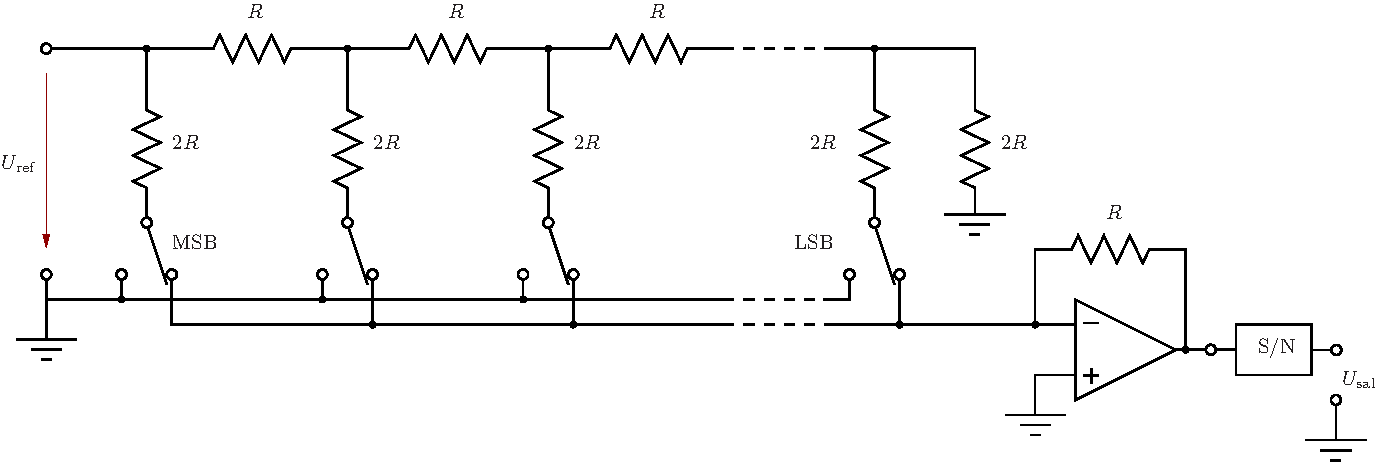
\includegraphics[width=0.9\textwidth]{ltxfig_prototipo}
  \caption{Ejemplo de imagen ltxfig/psfrag}
  \label{fig:ltxfig}
\end{figure}

\subsubsection{Figuras pstricks}  

\index{pstricks}
Los archivos con extensión \texttt{.pstricks} en el directorio \texttt{fig} se
utilizan para generar cualquier tipo de imágenes según el código que se
contenga.  Es un concepto más general que el anterior.  La
figura~\ref{fig:pstricks} ha sido creada con este esquema.  Puede revisar los
archivos \texttt{prototipo\_gnuplot*} como un ejemplo de su uso, en donde de un
archivo gnuplot (\texttt{\_.gp}) se genera un archivo \texttt{\_.eps}, el cual
es incluido en el archivo \texttt{.pstricks} sustituyendo cadenas de texto por
código LaTeX.

\begin{figure}[htb]
  \centering
  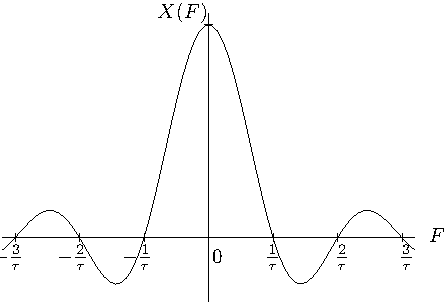
\includegraphics{prototipo_gnuplot}
  \caption{Ejemplo de imagen gnuplot/pstricks}
  \label{fig:pstricks}
\end{figure}

\subsubsection{Entradas en el índice de figuras}

El índice de figuras debe servir para encontrar rápidamente dónde se encuentra
cierta figura.  El pie de la figura, indicado en \LaTeX con \texttt{caption}
puede ser extenso, en especial para indicar detalles de las figura, y es la
entrada por defecto que aparecerá en el índice de figuras, la cual no debe
superar la extensión de una línea y debe únicamente dar la idea del contenido
de la figura para poder ser encontrada.  Para lograr esto en \LaTeX se utiliza
\begin{verbatim}
  \caption[Texto en el índice]{Texto al pie de la figura}
\end{verbatim}

\subsection{Referencias bibliográficas}

\index{referencias}\index{BibTeX}
Todo concepto o idea tomado de otros autores contar con la respectiva
referencia. En redacción técnica de ingeniería rara vez se utiliza la cita
textual, así que es necesario reformular las ideas y conceptos con palabras
propias. En ingeniería electrónica se utilizan los formatos de referencia de la
IEEE o la ACM, que son numéricos, encerrados entre paréntesis cuadrados (por
ejemplo, ``En \cite{Davis1963} se propuso un nuevo algoritmo'', o ``En
\cite{ProakisManolakis1998} los autores proponen tomar las ventajas de los
algorimos presentados en \cite{Oppenheim1998,Roberts2005,Haykin2001} por medio
del método de Newton \cite{Burrus1998} conocido en el área de optimización
lineal.''). La referencia es parte de las frases, así que si la frase termina
con la referencia para indicar la idea, ésta debe estar antes del punto final o
demás signos de puntuación: ``La capacidad de memoria también sigue una Ley
similar a la de Moore \cite{Octave}. Los siguientes son los aspectos a tomar en
cuenta en el diseño del sistema \cite{Lindner2002}:''

Se recomienda utilizar BibTeX para administrar las referencias bibliográficas.

\subsection{Extensión}

\index{extensión}
Una tesis de licenciatura no debe sobrepasar las 120 páginas incluyendo
apéndices y los formalismos desde portada hasta índices.

El cuerpo de la tesis (desde introducción hasta conclusiones) usualmente se
extiende desde 45 páginas hasta no más de 80, dependiendo de la problemática
tratada.

No es necesario reproducir contenidos de otras fuentes: agregue las referencias
a dichas fuentes, y limítese a enunciar lo estrictamente necesario para
comprender sus propuestas de solución.

\section{Sobre esta plantilla \LaTeX}

Esta plantilla \LaTeX pretende simplificar varios pasos en la creación del
documento de tesis.

\subsection{Marcar asuntos pendientes}

La plantilla tiene dos ``\emph{modos}'' de operación: normal y borrador
(\emph{draft}).  En el archivo \texttt{main.tex} a partir de la línea 41 usted
encuentra el código

\begin{verbatim}
%
% DRAFT MODE
%
\newboolean{draftmode}                  % boolean used to control draft-mode
% Ensure that only one of the next two lines is active:
\setboolean{draftmode}{true}            % turn draft mode on
%\setboolean{draftmode}{false}           % turn draft mode off
\end{verbatim}

Con el modo borrador, se activan ciertos comandos y funcionalidades útiles en
el proceso de elaboración de la tesis, pero que deben ser desactivados al
final, antes de entregar la tesis.  Por ejemplo, se activa el pie de página que
dice ``\emph{Borrador: fecha}'', y se activa el índice titulado ``Revisar''.  En dicho índice aparecen las páginas en donde se hayan utilizado alguno de los siguientes comandos:
\begin{compactitem}
\item \verb+\boxcomment{comentario}+ Crea una caja en el margen de página con
  el comentario indicado.
\item \verb+\explain{comentario}+ Crea una caja en el margen de página con
  el comentario indicado, con una flecha hacia la derecha para indicar qué en
  concreto debe ser revisado.
\item \verb+\chk{comentario}+ Crea una caja en el margen con símbolo de
  ``chequeado'' y el comentario indicado.
\item \verb+\TODO{comentario}+ Crea una caja grande de fondo sombreado con el
  comentario indicado.
\end{compactitem}

En este párrafo se\chk{resultado de chk} utilizan algunos de estos comandos
para ilustrar su efecto.  El \verb+\chk+ como puede observar tiene sentido
usarlo para marcar que algo está casi listo.  Por otro lado \explain{explain}
el comando \verb+\explain+ permite marcar algo que requiere ser revisado en
redacción, valores, etc.  El \verb+\boxcomment+\boxcomment{La caja simple}
solo pone una marca al margen.

\TODO{Finalmente el comando \texttt{TODO} coloca esta caja gris.}

Si usted desativa el modo draft, desaparecen todas las páginas, y desaparece el
índice ``Revisar''.  En éste índice aparecen todas las páginas en donde se
utilizaron estos comandos con los respectivos comentarios, lo que permite
encontrar rápidamente detalles que usted indicó que debe revisar.

\subsection{Índices}

Como índice se conoce la lista de términos claves con su respectiva página, al
final del documento.  La plantilla ofrece varios comandos para simplificar el
uso estandar del comando de \LaTeX\ \verb+\index{termino}+ que coloca al término
indicado en el índice.  Con \verb+\nt[indice]{termino}+ (\emph{new term}) usted
indica la entrada principal del término, que aparece en el texto en el índice,
es decir, en el índice aparece lo que indique en vez de ``indice'' y en el
texto aparece lo que indique ``termino''; \verb+\ot{termino}+ agrega una
entrada secundaria al término.
